\begin{figure}[H]
	\centering
	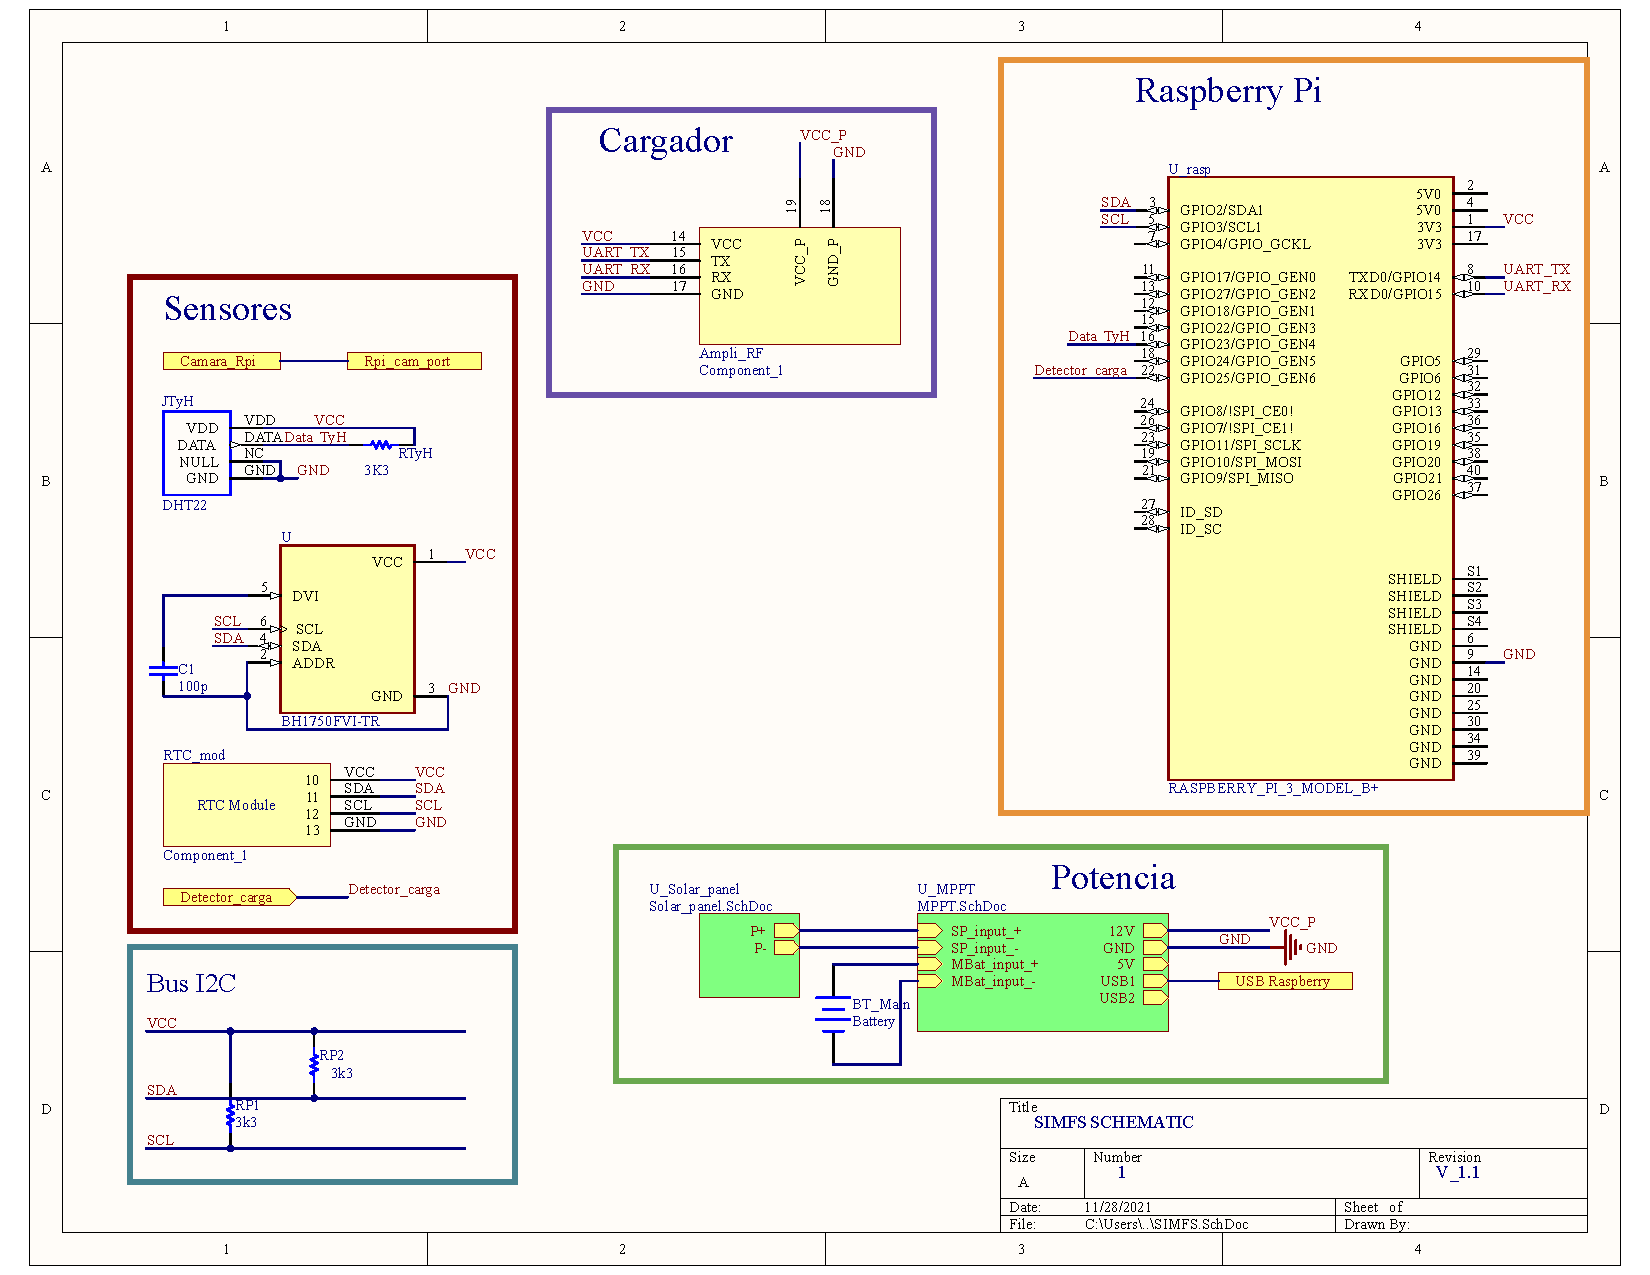
\includegraphics[width=0.9\linewidth]{ImagenesApendice/esquematico}
	\caption{Esquemático de conexionado del \textit{shield}.}
	\label{fig:esquematico_conexionado_1}
\end{figure}

\begin{figure}[H]
	\centering
	\includegraphics[width=0.9\linewidth]{ImagenesApendice/esquematicoSensores}
	\caption{Esquemático de conexionado para la placa de sensores.}
	\label{fig:esquematico_conexionado_2}
\end{figure}

\begin{figure}[H]
	\centering
	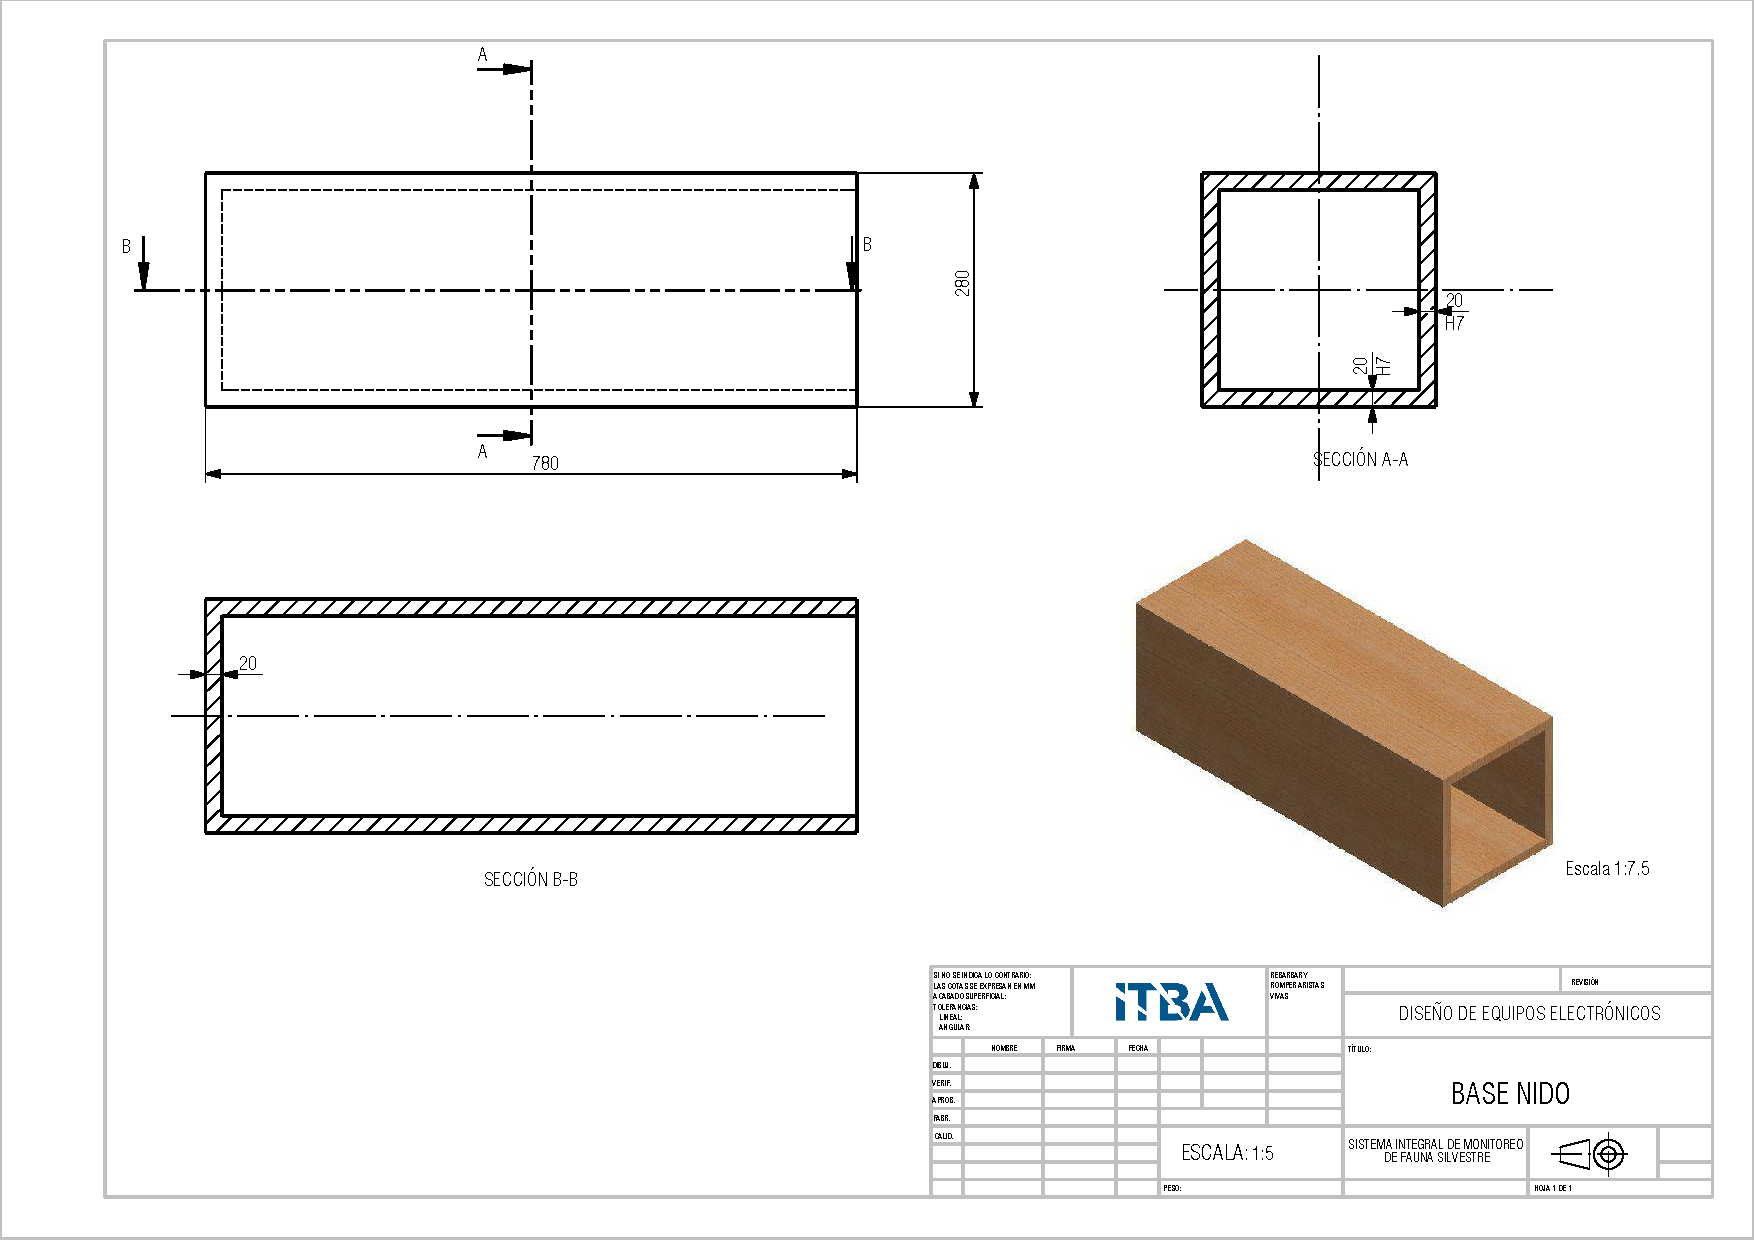
\includegraphics[width=\linewidth]{ImagenesApendice/Base_nido_plano}
	\caption{Plano de la base del prototipo de nido.}
	\label{fig:base_nido_plano}
\end{figure}

%\begin{figure}[H]
%	\centering
%	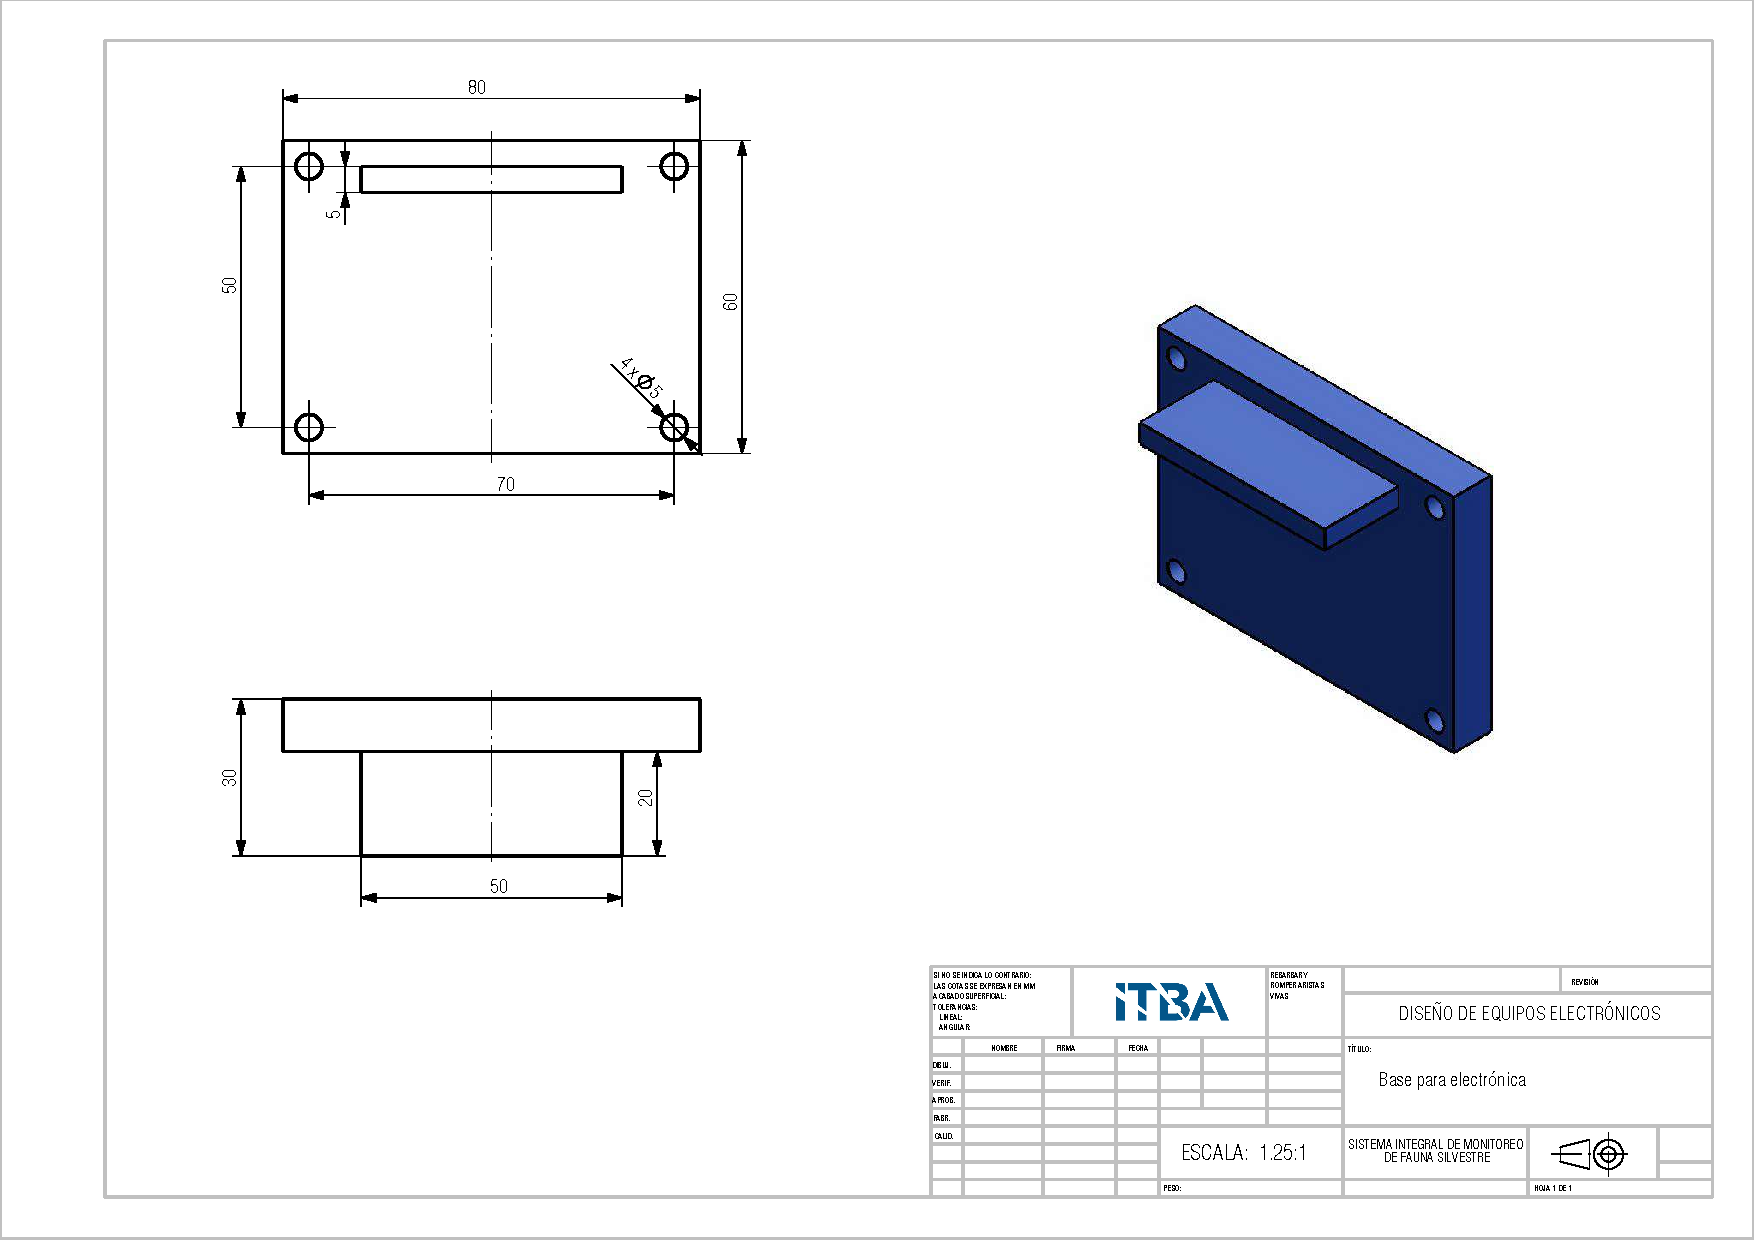
\includegraphics[width=\linewidth]{ImagenesApendice/Base_electronica_plano}
%	\caption{Plano de la base para la electrónica prototipo.}
%	\label{fig:base_electronica_plano}
%\end{figure}

\begin{figure}[H]
	\centering
	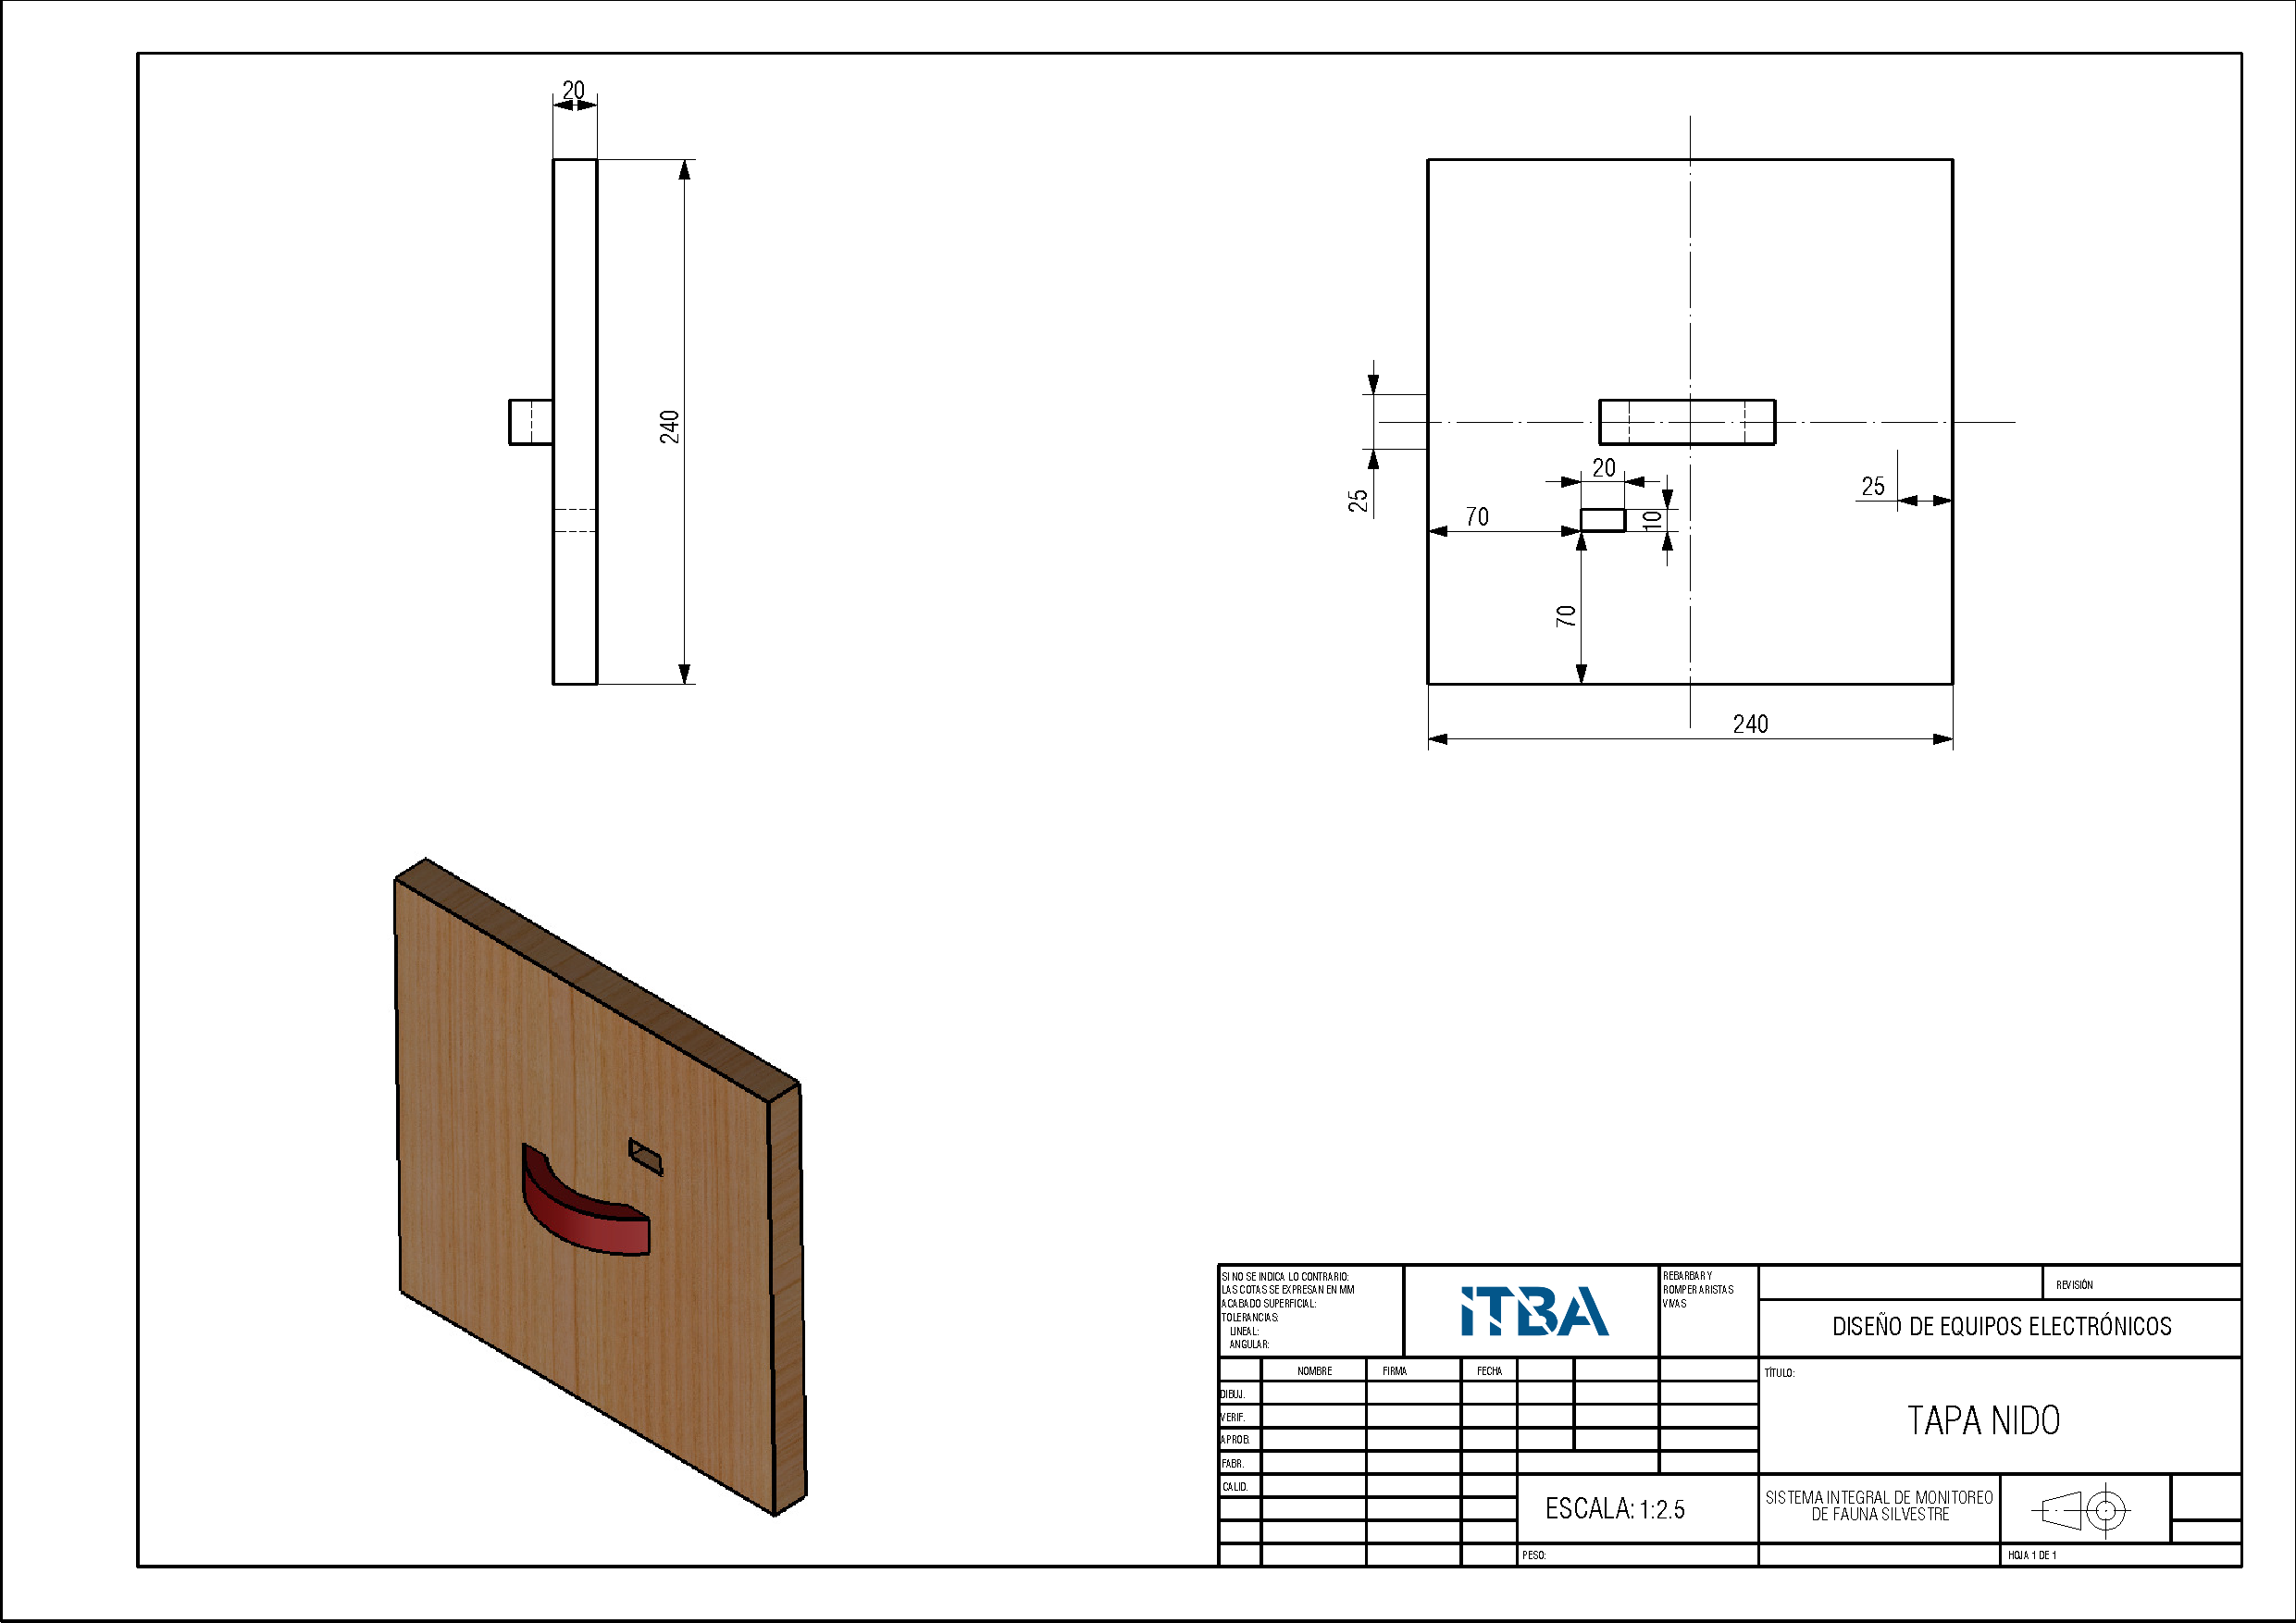
\includegraphics[width=\linewidth]{ImagenesApendice/tapa_nido_plano}
	\caption{Plano de la tapa del prototipo de nido.}
	\label{fig:tapa_nido_plano}
\end{figure}

\begin{figure}[H]
	\centering
	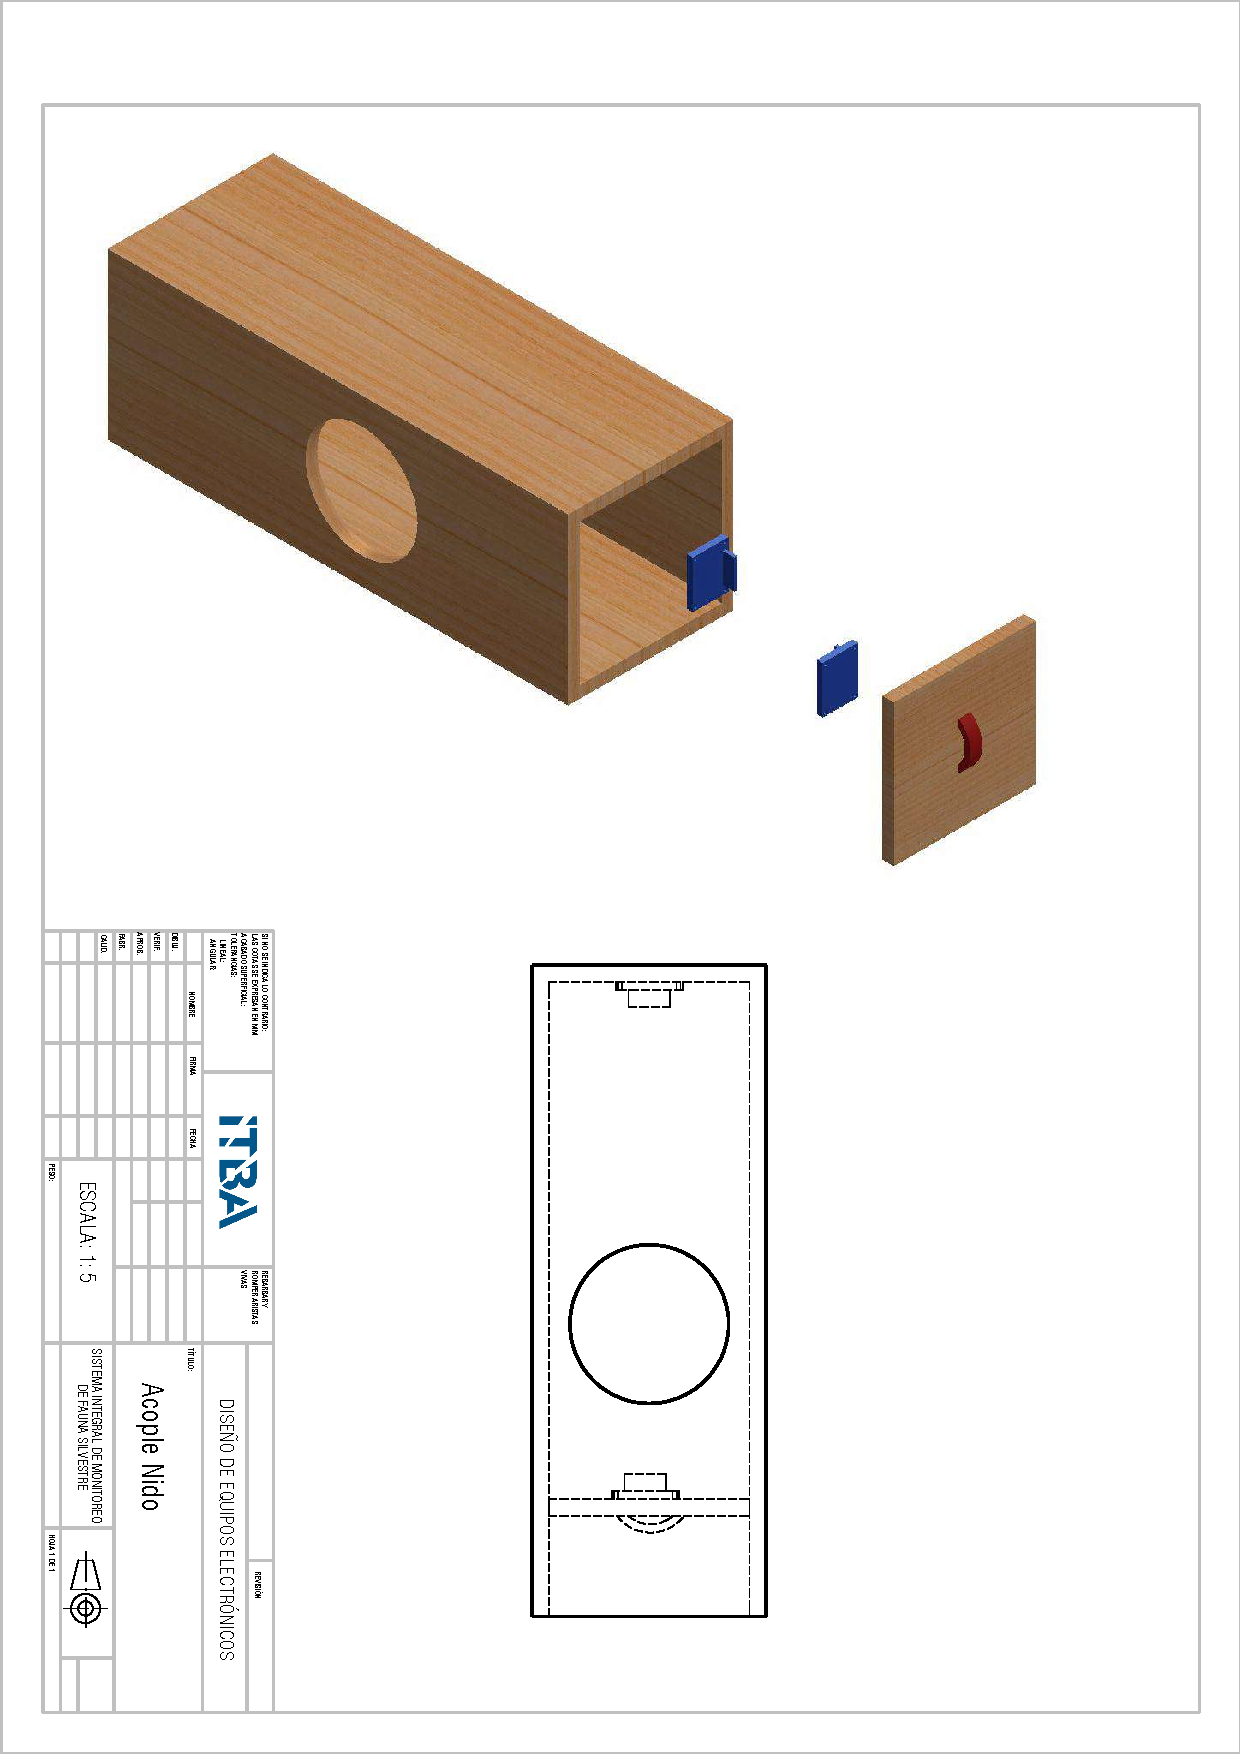
\includegraphics[width=\linewidth]{ImagenesApendice/explotado_nido}
	\caption{Plano explotado del prototipo.}
	\label{fig:explotado_nido_plano}
\end{figure}

\begin{figure}[H]
	\centering
	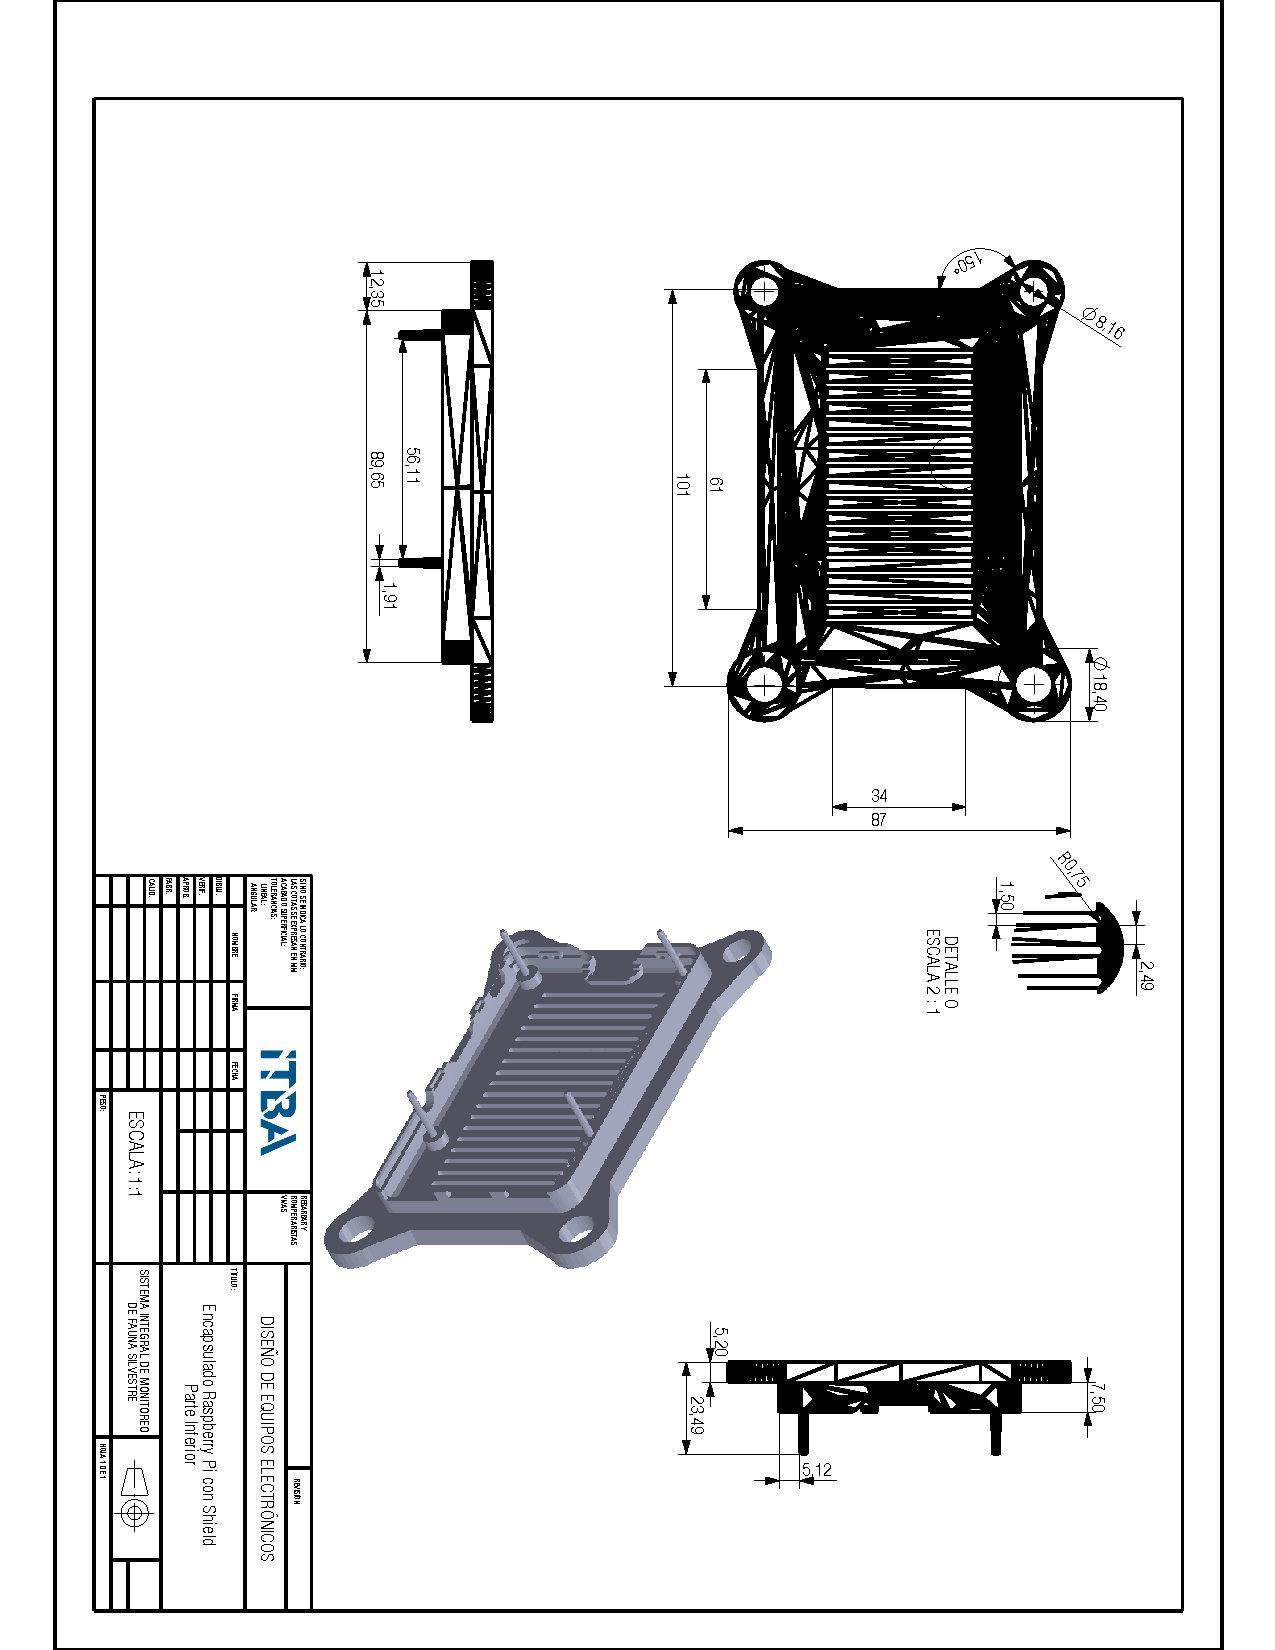
\includegraphics[width=\linewidth]{ImagenesApendice/RpiCasingBottom}
	\caption{Plano del encapsulado para la Raspberry Pi con Shield, encastre inferior.}
	\label{fig:RpiCasingBottom}
\end{figure}

\begin{figure}[H]
	\centering
	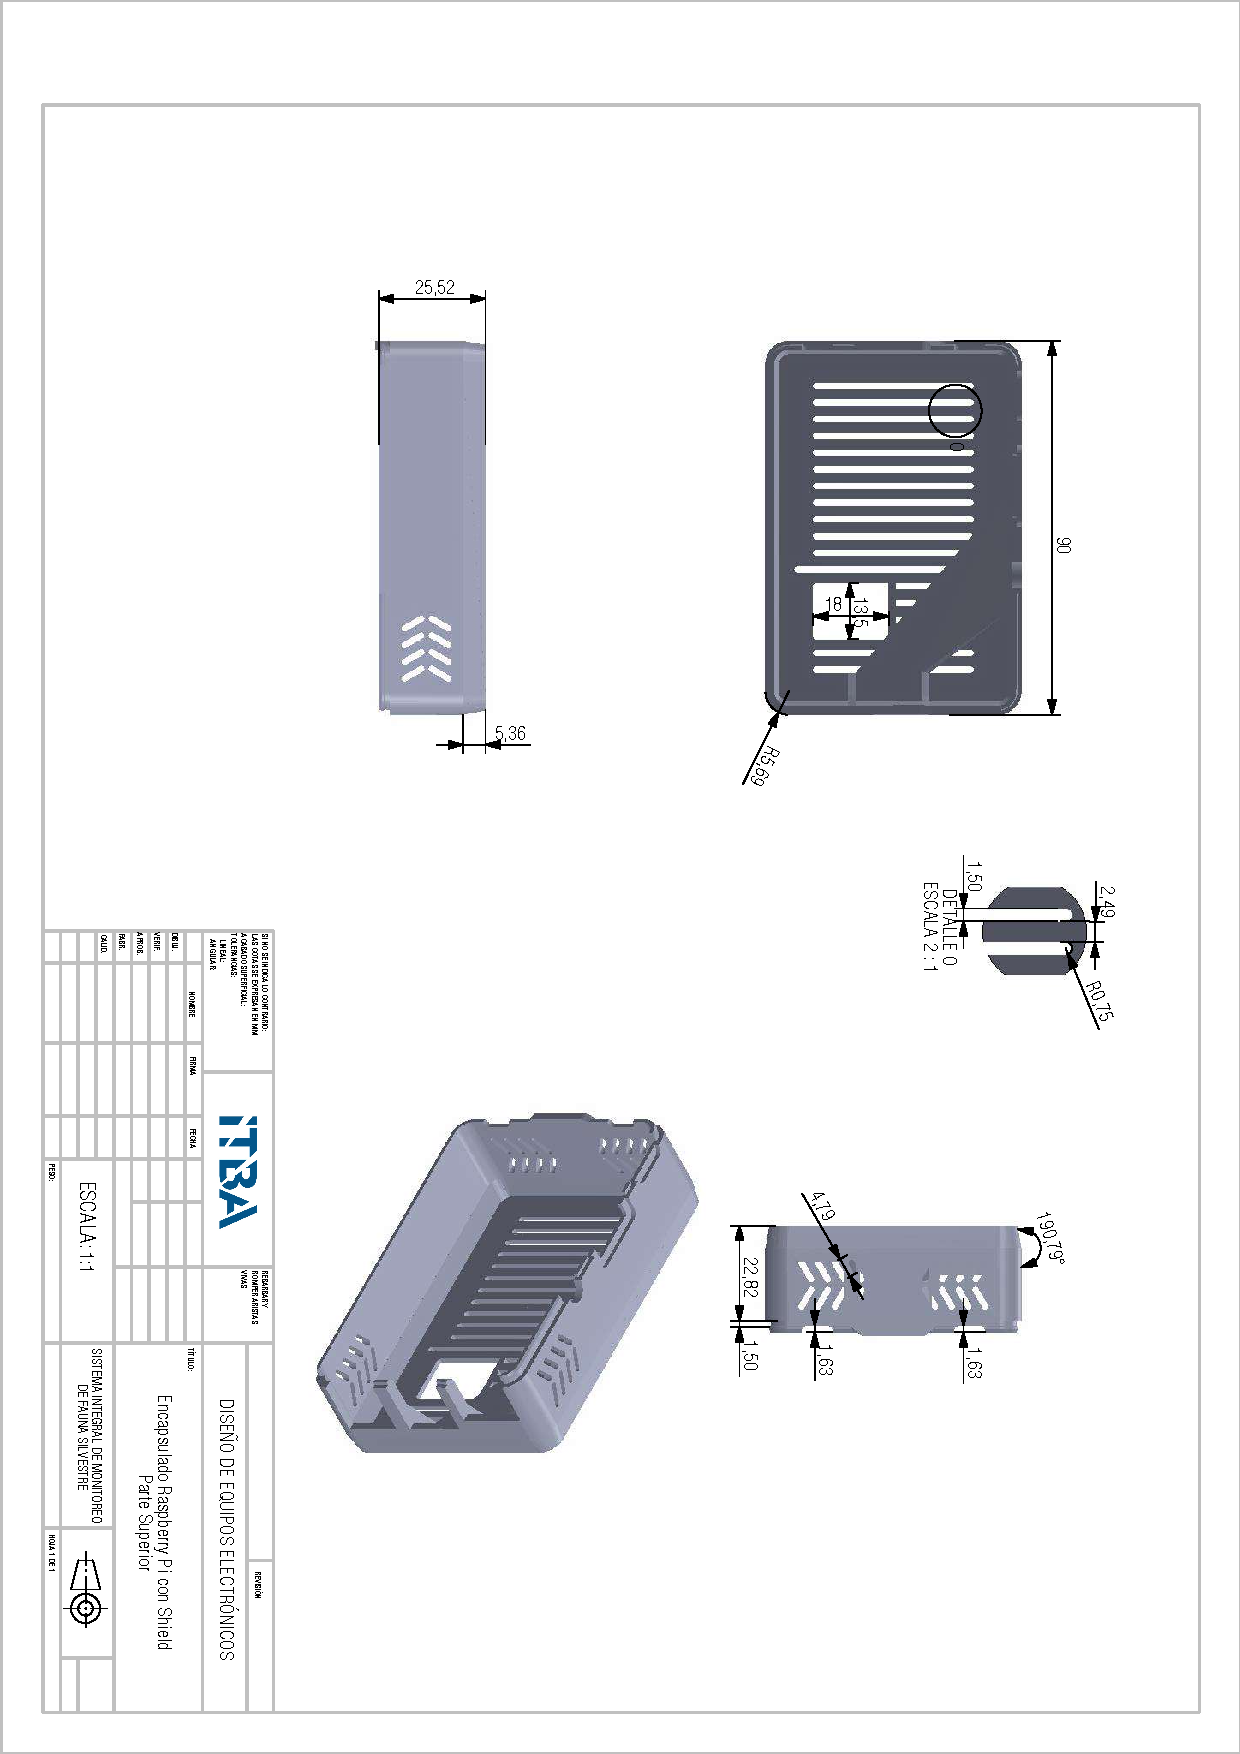
\includegraphics[width=\linewidth]{ImagenesApendice/RpiCasingTop}
	\caption{Plano del encapsulado para la Raspberry Pi con Shield, encastre superior.}
	\label{fig:RpiCasingTop}
\end{figure}